\thispagestyle{fancy}
\vspace*{40 pt}
\subsection{Tela comando impressora}
 Esta tela é acessada pelo botão "\textgreater" no menu superior esquerdo da tela de comando alimentação, no mesmo da tela comandos de uma impressora anterior (se ouver),pelo botão de atalho da tela de comando das
\textbf{impressoras}, pelo botão "\textless{}" no menu superior esquerdo da tela comando impressora posterior (se ouver) ou slotter quando não tiver nenhuma impressora a mais, pelo atalho na tela de comando das \textbf{impressoras} e pelo botão comando da tela ajustes impressora.
\vspace*{\fill}
\begin{figure}[h]
  \centering
  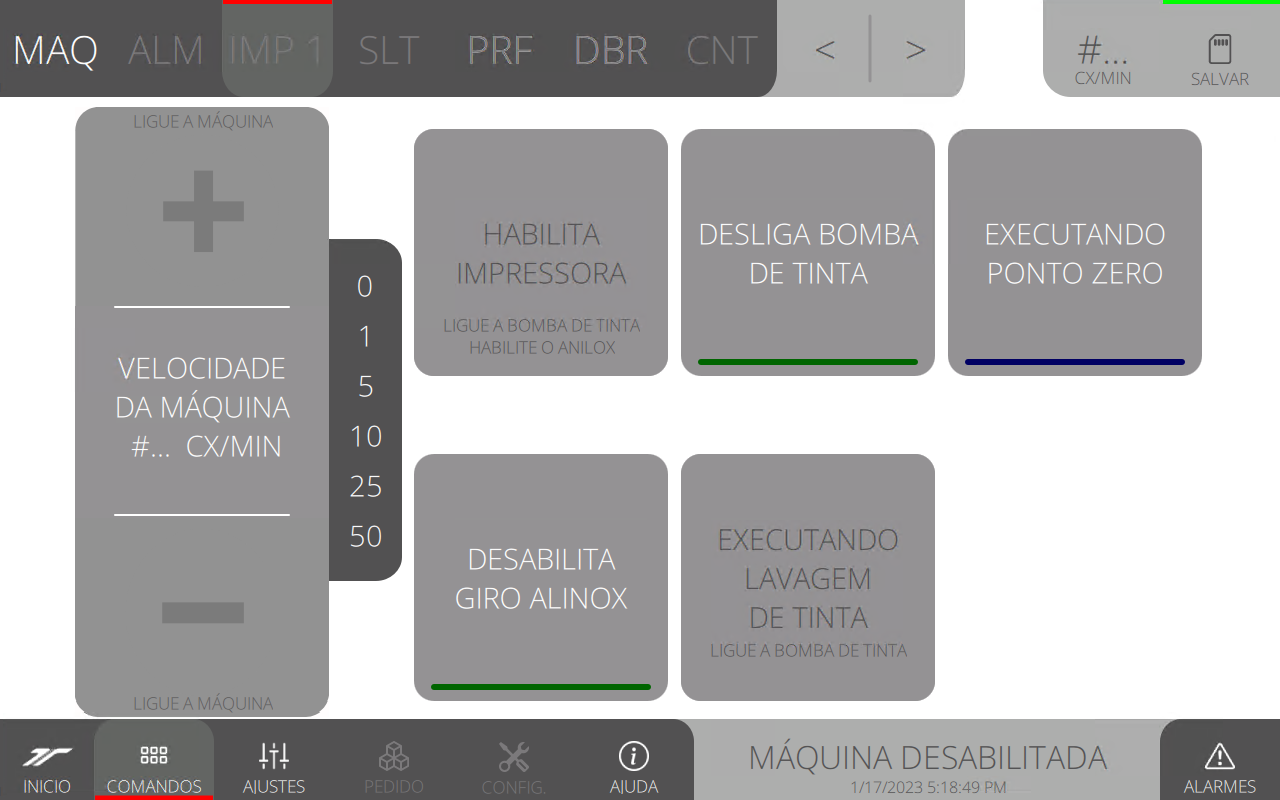
\includegraphics[width=576px,height=360px]{src/imagesFlexo/04-printter/02-printter/commands/e-Tela-Principal.png}
\end{figure}
\vspace*{\fill}

\newpage
\thispagestyle{fancy}
\vspace*{40 pt}
\subsubsection{\small{Executa lavagem de tinta}}
\vspace*{\fill}
\begin{figure}[h]
  \centering
  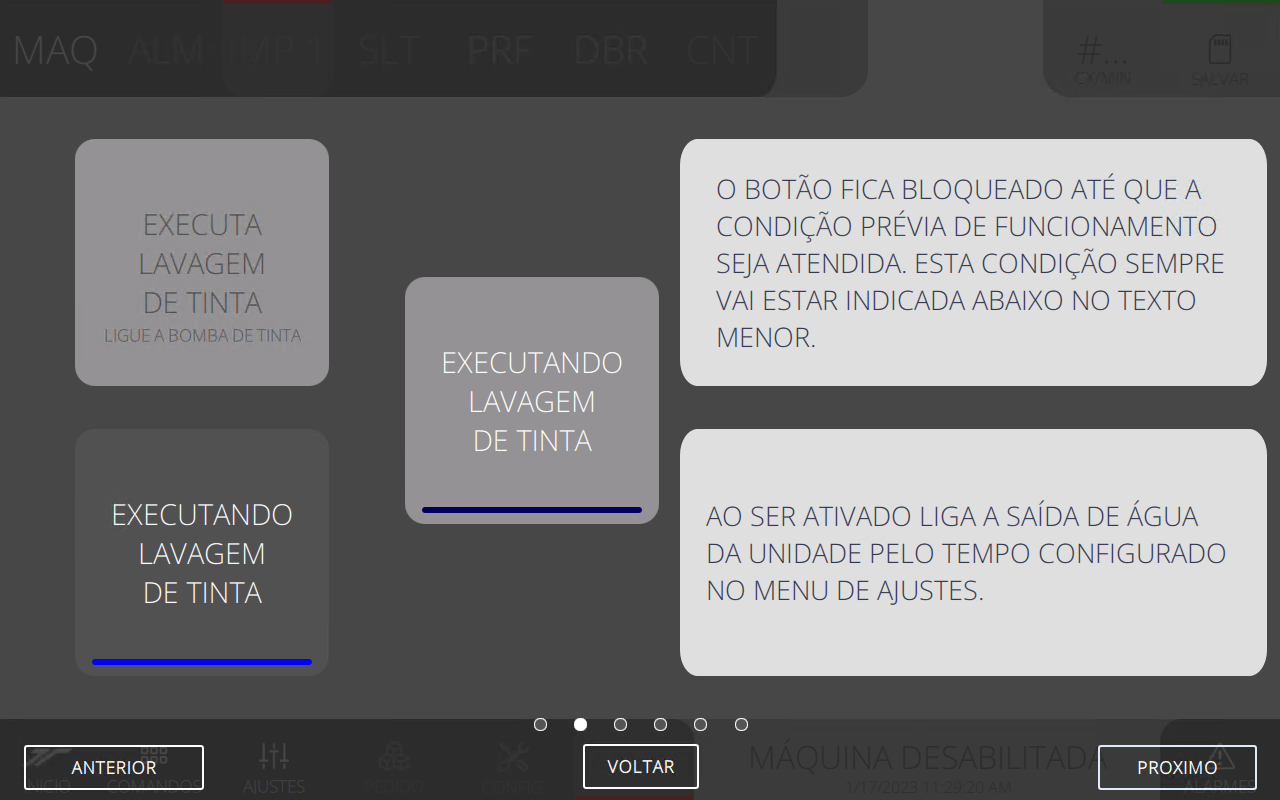
\includegraphics[width=576px,height=360px]{src/imagesFlexo/04-printter/02-printter/commands/e-2.png}
\end{figure}
\vspace*{\fill}

\newpage
\thispagestyle{fancy}
\vspace*{40 pt}
\subsubsection{\small{Habilita giro anilox}}
\vspace*{\fill}
\begin{figure}[h]
  \centering
  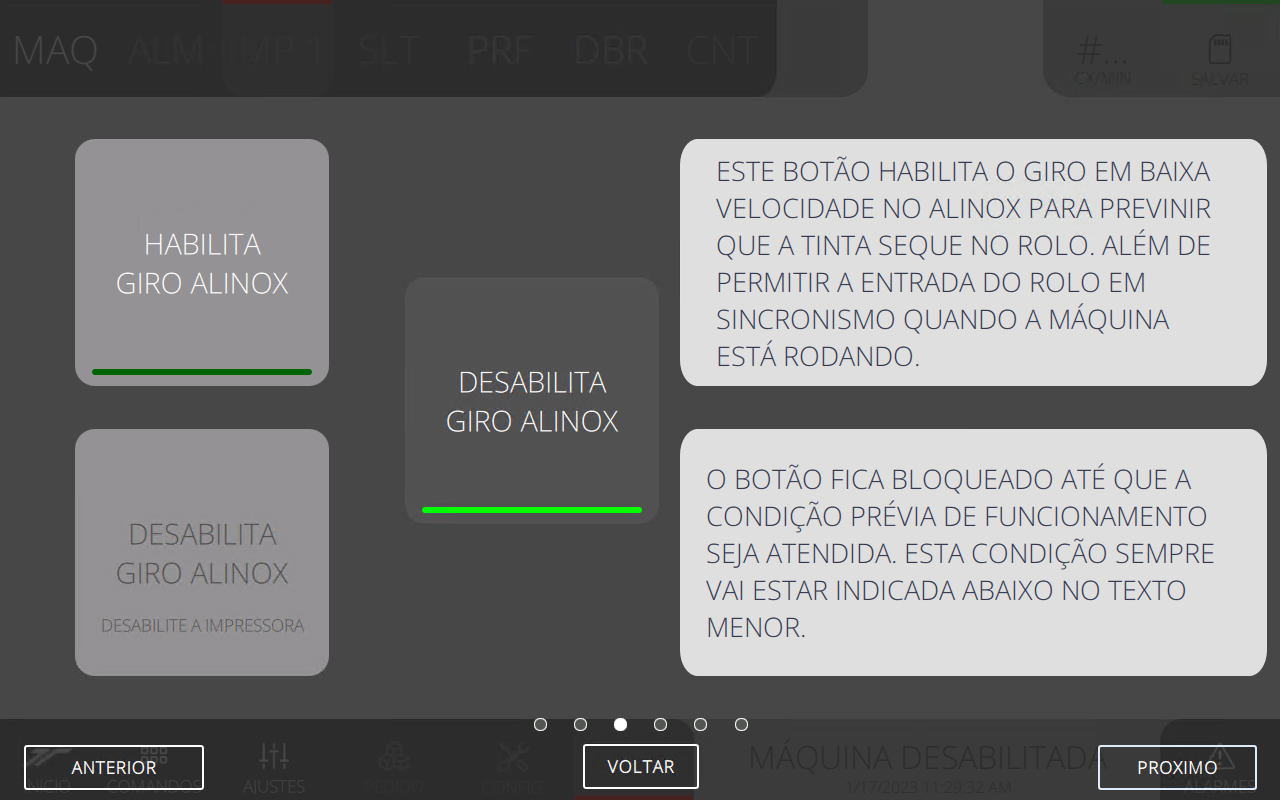
\includegraphics[width=576px,height=360px]{src/imagesFlexo/04-printter/02-printter/commands/e-3.png}
\end{figure}
\vspace*{\fill}

\newpage
\thispagestyle{fancy}
\vspace*{40 pt}
\subsubsection{\small{Executa ponto zero}}
\vspace*{\fill}
\begin{figure}[h]
  \centering
  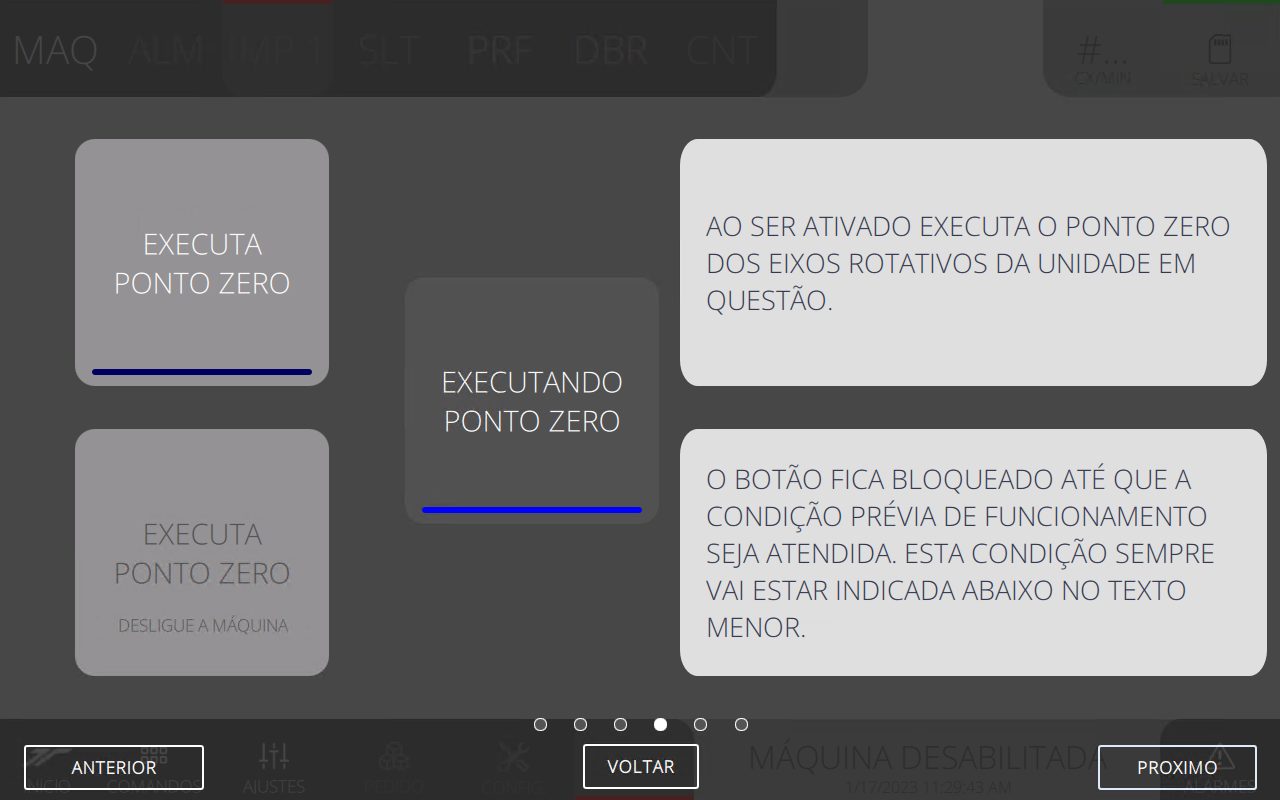
\includegraphics[width=576px,height=360px]{src/imagesFlexo/04-printter/02-printter/commands/e-4.png}
\end{figure}
\vspace*{\fill}

\newpage
\thispagestyle{fancy}
\vspace*{40 pt}
\subsubsection{\small{Liga bomba de tinta}}
\vspace*{\fill}
\begin{figure}[h]
  \centering
  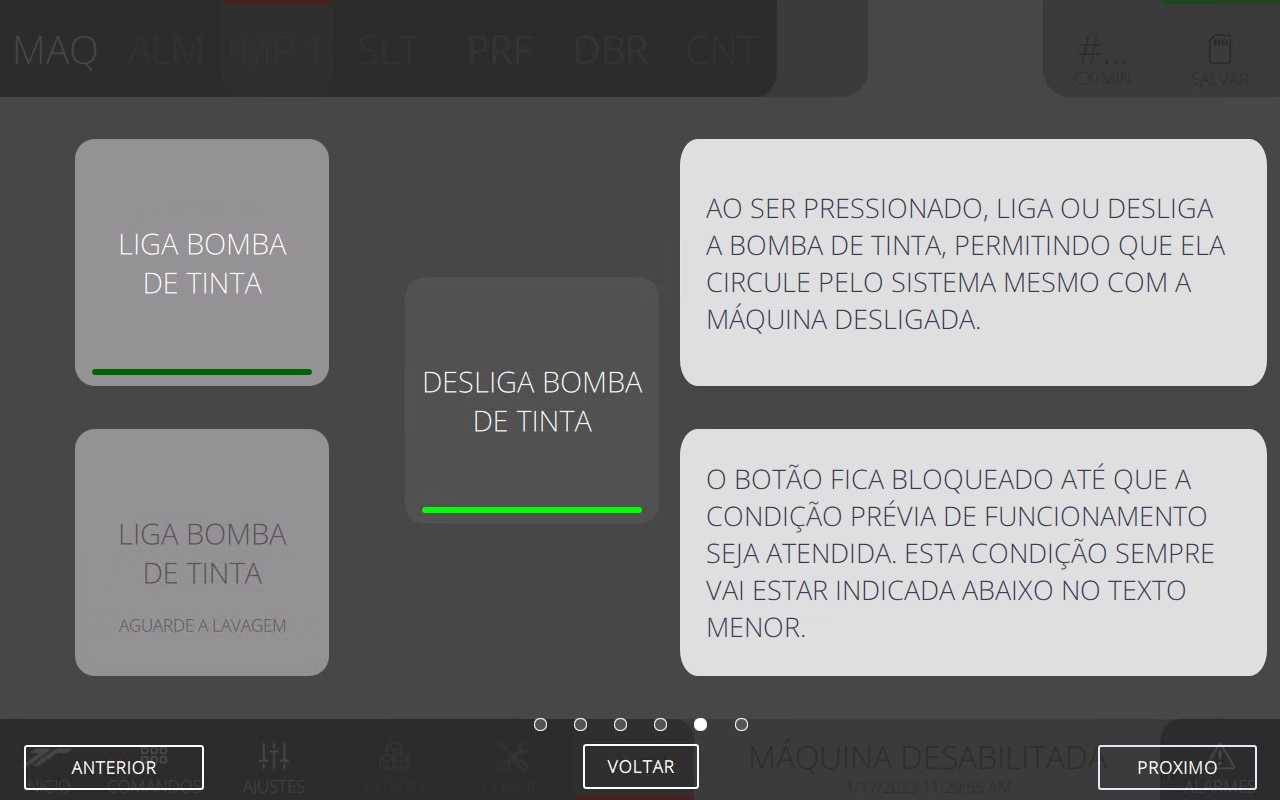
\includegraphics[width=576px,height=360px]{src/imagesFlexo/04-printter/02-printter/commands/e-5.png}
\end{figure}
\vspace*{\fill}

\newpage
\thispagestyle{fancy}
\vspace*{40 pt}
\subsubsection{\small{Desabilita impressora}}
\vspace*{\fill}
\begin{figure}[h]
  \centering
  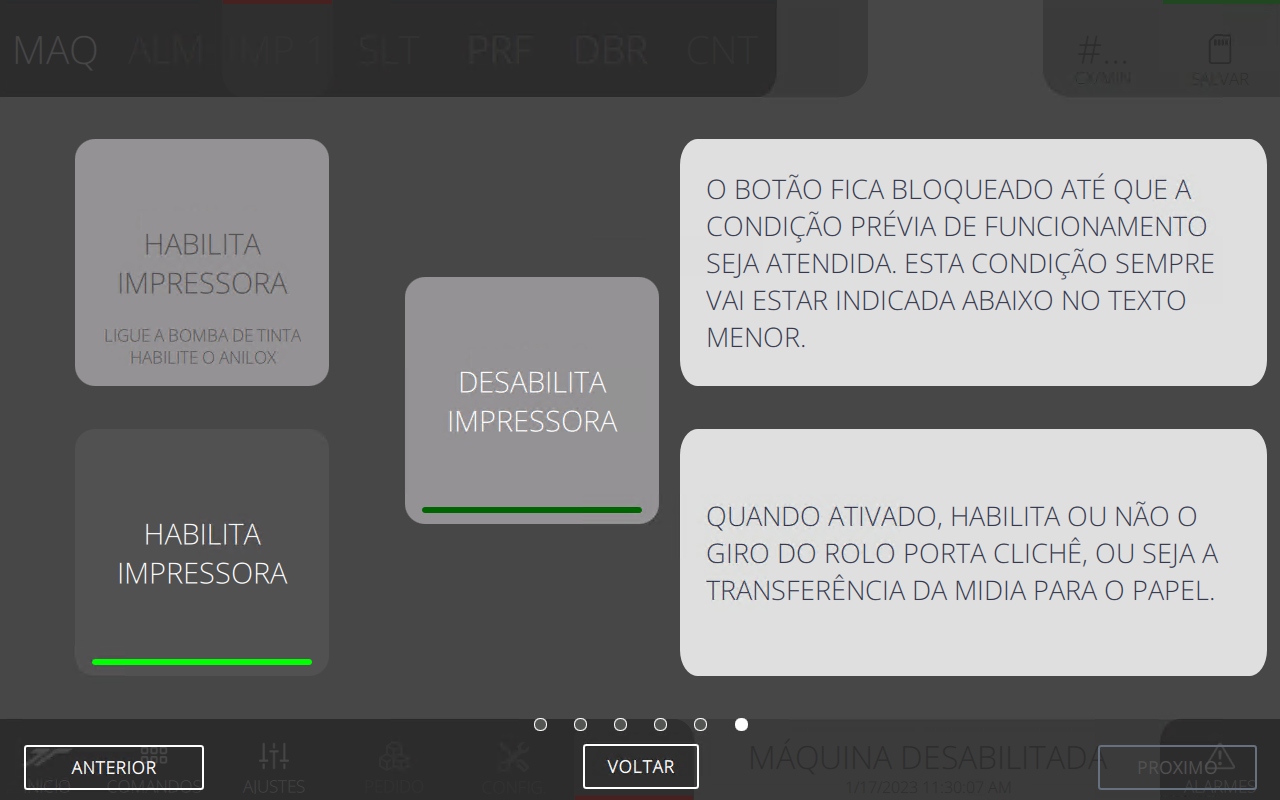
\includegraphics[width=576px,height=360px]{src/imagesFlexo/04-printter/02-printter/commands/e-6.png}
\end{figure}
\vspace*{\fill}